%Notes by Harsh Mistry 
%CS 444
%based on Template from : https://www.cs.cmu.edu/~ggordon/10725-F12/template.tex

\documentclass{article}
\setlength{\oddsidemargin}{0.25 in}
\setlength{\evensidemargin}{-0.25 in}
\setlength{\topmargin}{-0.6 in}
\setlength{\textwidth}{6.5 in}
\setlength{\textheight}{8.5 in}
\setlength{\headsep}{0.75 in}
\setlength{\parindent}{0 in}
\setlength{\parskip}{0.1 in}
\usepackage{amsfonts,graphicx, amssymb}
\usepackage[fleqn]{amsmath}
\usepackage{fixltx2e}
\usepackage{color}
\usepackage{tcolorbox}
\usepackage{lipsum}
\usepackage{listings}
\graphicspath{ {./images/} }
\usepackage{scrextend}
\tcbuselibrary{skins,breakable}
\usetikzlibrary{shadings,shadows}
\newcounter{lecnum}
\renewcommand{\thepage}{\thelecnum-\arabic{page}}
\renewcommand{\thesection}{\thelecnum.\arabic{section}}
\renewcommand{\theequation}{\thelecnum.\arabic{equation}}
\renewcommand{\thefigure}{\thelecnum.\arabic{figure}}
\renewcommand{\thetable}{\thelecnum.\arabic{table}}
\newcommand{\lecture}[4]{
   \pagestyle{myheadings}
   \thispagestyle{plain}
   \newpage
   \setcounter{lecnum}{#1}
   \setcounter{page}{1}
   
   
%Info Box 
   \begin{center}
   \framebox{
      \vbox{\vspace{2mm}
    \hbox to 6.28in { {\bf CS 444 - Compiler Construction 
	\hfill Winter 2020} }
       \vspace{4mm}
       \hbox to 6.28in { {\Large \hfill Lecture #1: #2  \hfill} }
       \vspace{2mm}
       \hbox to 6.28in { {\it Lecturer: #3 \hfill Notes By: #4} }
      \vspace{2mm}}
   }
   \end{center}
   
   \markboth{Lecture #1: #2}{Lecture #1: #2}



 
}

\renewcommand{\cite}[1]{[#1]}
\def\beginrefs{\begin{list}%
        {[\arabic{equation}]}{\usecounter{equation}
         \setlength{\leftmargin}{2.0truecm}\setlength{\labelsep}{0.4truecm}%
         \setlength{\labelwidth}{1.6truecm}}}
\def\endrefs{\end{list}}
\def\bibentry#1{\item[\hbox{[#1]}]}

\newcommand{\fig}[3]{
			\vspace{#2}
			\begin{center}
			Figure \thelecnum.#1:~#3
			\end{center}
	}
	
\newcommand{\pipe}{\(\mid\)}
\newcommand{\ctr}{\(\wedge\)}

\newtheorem{theorem}{Theorem}[lecnum]
\newtheorem{lemma}[theorem]{Lemma}
\newtheorem{ex}[theorem]{Example}
\newtheorem{proposition}[theorem]{Proposition}
\newtheorem{claim}[theorem]{Claim}
\newtheorem{corollary}[theorem]{Corollary}
\newtheorem{definition}[theorem]{Definition}
\newenvironment{proof}{{\bf Proof:}}{\hfill\rule{2mm}{2mm}}
\newcommand\E{\mathbb{E}}

%color definitions :
\definecolor{darkred}{rgb}{0.55, 0.0, 0.0}
\definecolor{lightcoral}{rgb}{0.94, 0.5, 0.5}
\definecolor{tomato}{rgb}{1.0, 0.39, 0.28}
\definecolor{lightgray}{rgb}{.9,.9,.9}
\definecolor{darkgray}{rgb}{.4,.4,.4}
\definecolor{purple}{rgb}{0.65, 0.12, 0.82}
\definecolor{lightgreen}{rgb}{0.56, 0.93, 0.56}
\definecolor{darkgreen}{rgb}{0.0, 0.2, 0.13}
\definecolor{limegreen}{rgb}{0.2, 0.8, 0.2}
\definecolor{lightblue}{rgb}{0.68, 0.85, 0.9}
\definecolor{darkblue}{rgb}{0.0, 0.0, 0.55}


%Environments
\newenvironment{exblock}[1]{%
    \tcolorbox[beamer,%
    noparskip,breakable,
    colback=lightgreen,colframe=darkgreen,%
    colbacklower=limegreen!75!lightgreen,%
    title=#1]}%
    {\endtcolorbox}

\newenvironment{ablock}[1]{%
    \tcolorbox[beamer,%
    noparskip,breakable,
    colback=lightcoral,colframe=darkred,%
    colbacklower=tomato!75!lightcoral,%
    title=#1]}%
    {\endtcolorbox}

\newenvironment{cblock}[1]{%
    \tcolorbox[beamer,%
    noparskip,breakable,
    colback=lightblue,colframe=darkblue,%
    colbacklower=darkblue!75!lightblue,%
    title=#1]}%
    {\endtcolorbox}


%Languages
\lstdefinelanguage{JavaScript}{
  keywords={typeof, new, true, false, catch, function, return, null, catch, switch, var, if, in,  fi, while, do, else, case, break},
  keywordstyle=\color{blue}\bfseries,
  ndkeywords={class, export, boolean, throw, implements, import, this},
  ndkeywordstyle=\color{darkgray}\bfseries,
  identifierstyle=\color{black},
  sensitive=false,
  comment=[l]{//},
  morecomment=[s]{/*}{*/},
  commentstyle=\color{purple}\ttfamily,
  stringstyle=\color{red}\ttfamily,
  morestring=[b]',
  morestring=[b]"
}

%Listings
\lstset{
   language=JavaScript,
   backgroundcolor=\color{lightgray},
   extendedchars=true,
   basicstyle=\footnotesize\ttfamily,
   showstringspaces=false,
   showspaces=false,
   numbers=left,
   numberstyle=\footnotesize,
   numbersep=9pt,
   tabsize=2,
   breaklines=true,
   showtabs=false,
   captionpos=b
}

\newcommand*\circled[1]{\tikz[baseline=(char.base)]{
            \node[shape=circle,draw,inner sep=2pt] (char) {#1};}}

%Start of Document 
\begin{document}

\lecture{11}{February 10th , 2020}{Ond\u{r}ej Lhot\'{a}k}{Harsh Mistry}



\section{Context-sensitive analysis continued}

\subsection{Name Resolution}

\begin{itemize}
\item Link each use of a name to a declaration
\item In Java : 
\textcolor{blue}{A2} and  \textcolor{red}{A3}
\begin{enumerate}
\color{blue}
\item Build global environment
\item Resolve type names
\item Build/check class hierarchy (methods/files)

\color{red}
\item Disambiguate ambiguous namespace 
\begin{itemize}
\item In Java you can't simply determine the namespace based on location of usage
\end{itemize} 
\item Resolve "expressions" (Variables, static fields)
\item Type checking
\item Resolve methods instance (non-static) fields
\end{enumerate}
\item (1) Building a global environment 
\begin{itemize}
\item Simply create a set of all classes with packages
\item Its important to note that the "default" package is NOT the root package 
\item There is no way to declare class that falls within the default package
\end{itemize}
\item (2)  Resolving type names \textcolor{orange}{(Refer to JLS 6.5)}
\begin{itemize}
\item Types
\begin{itemize}
\item Qualified Name (with dots) (i.e a.b.c)
\begin{itemize}
\item Must be full name of type 
\item No notion of relative path names
\end{itemize}
\item Simple Name (no dot) (c)
\end{itemize}
\item Resolving steps
\begin{enumerate}
\item Is it the enclosing class/interface?
\item Is it a single-type import (a.b.c)?
\item Is it a type in the current package (of the enclosing type)?
\item Is it a import-on-demand package (a.b.t)?
\end{enumerate}
\item Each step \circled{1} - \circled{4} must be unambiguous
\end{itemize}
\newpage
\item (3) Building and checking class hierarchy
\begin{itemize}
\item Simple Checks 
\begin{enumerate}
\item Class A extends B \(\implies\) B must be class  \textcolor{orange}{(Refer to JLS 8.1.3)}
\item Class A implements D \(implies\) D must be an interface \textcolor{orange}{(Refer to JLS 8.1.4)}
\item No duplicate interfaces (i.e \verb|Class E implements F,F|) \textcolor{orange}{(Refer to JLS 8.1.4)}
\item B cannot be final \textcolor{orange}{(Refer to JLS 8.1.3)}
\item Two constructors of the same class must have different signatures (Parameter Lists) \textcolor{orange}{(Refer to JLS 8.8.2)}
\end{enumerate}
\begin{definition} Super(A) = direct super-classes / interfaces of A\\
Examples
\begin{itemize}
\item Class A extends B implements C,D,E \(\implies\) super(A) = \(\{B, C, D, E\}\)
\item If unspecified, B is Java.lang.Object
\item super(Java.lang.Object) = \(\{\}\)
\item Interface F extends GHI 
\item super(F) = \(\{G,H, I \}\)
\end{itemize}
\end{definition}
\item Rules
\begin{itemize}
\item $$ \frac{T \in super(S)}{S < T}$$
\item $$ \frac{S < T }{S \leq T } $$
\item $$ \frac{}{T \leq T }$$
\item $$ \frac{S < T^\prime  \hspace{0.5cm} T^\prime < T }{S < T} $$
\item $$ S < T \implies \text{ S is a \underline{strict subtype} of T} $$
\end{itemize}
\begin{definition}-\\
\begin{itemize}
\item declare(T) = set of methods/fields in body of T
\item inherit(T) = m/f that T inherits 
\item contain(T) = declare(T) \(\cup\) inherit(T)
\item replace(\(m, m^\prime\)) 
\begin{itemize}
\item m "overrides" \(m^\prime\)
\item m "hides" \(m^\prime\)
\item f "hides" \(f^\prime\)
\end{itemize}
\end{itemize}
\end{definition}
\newpage
\item More Rules
\begin{center}
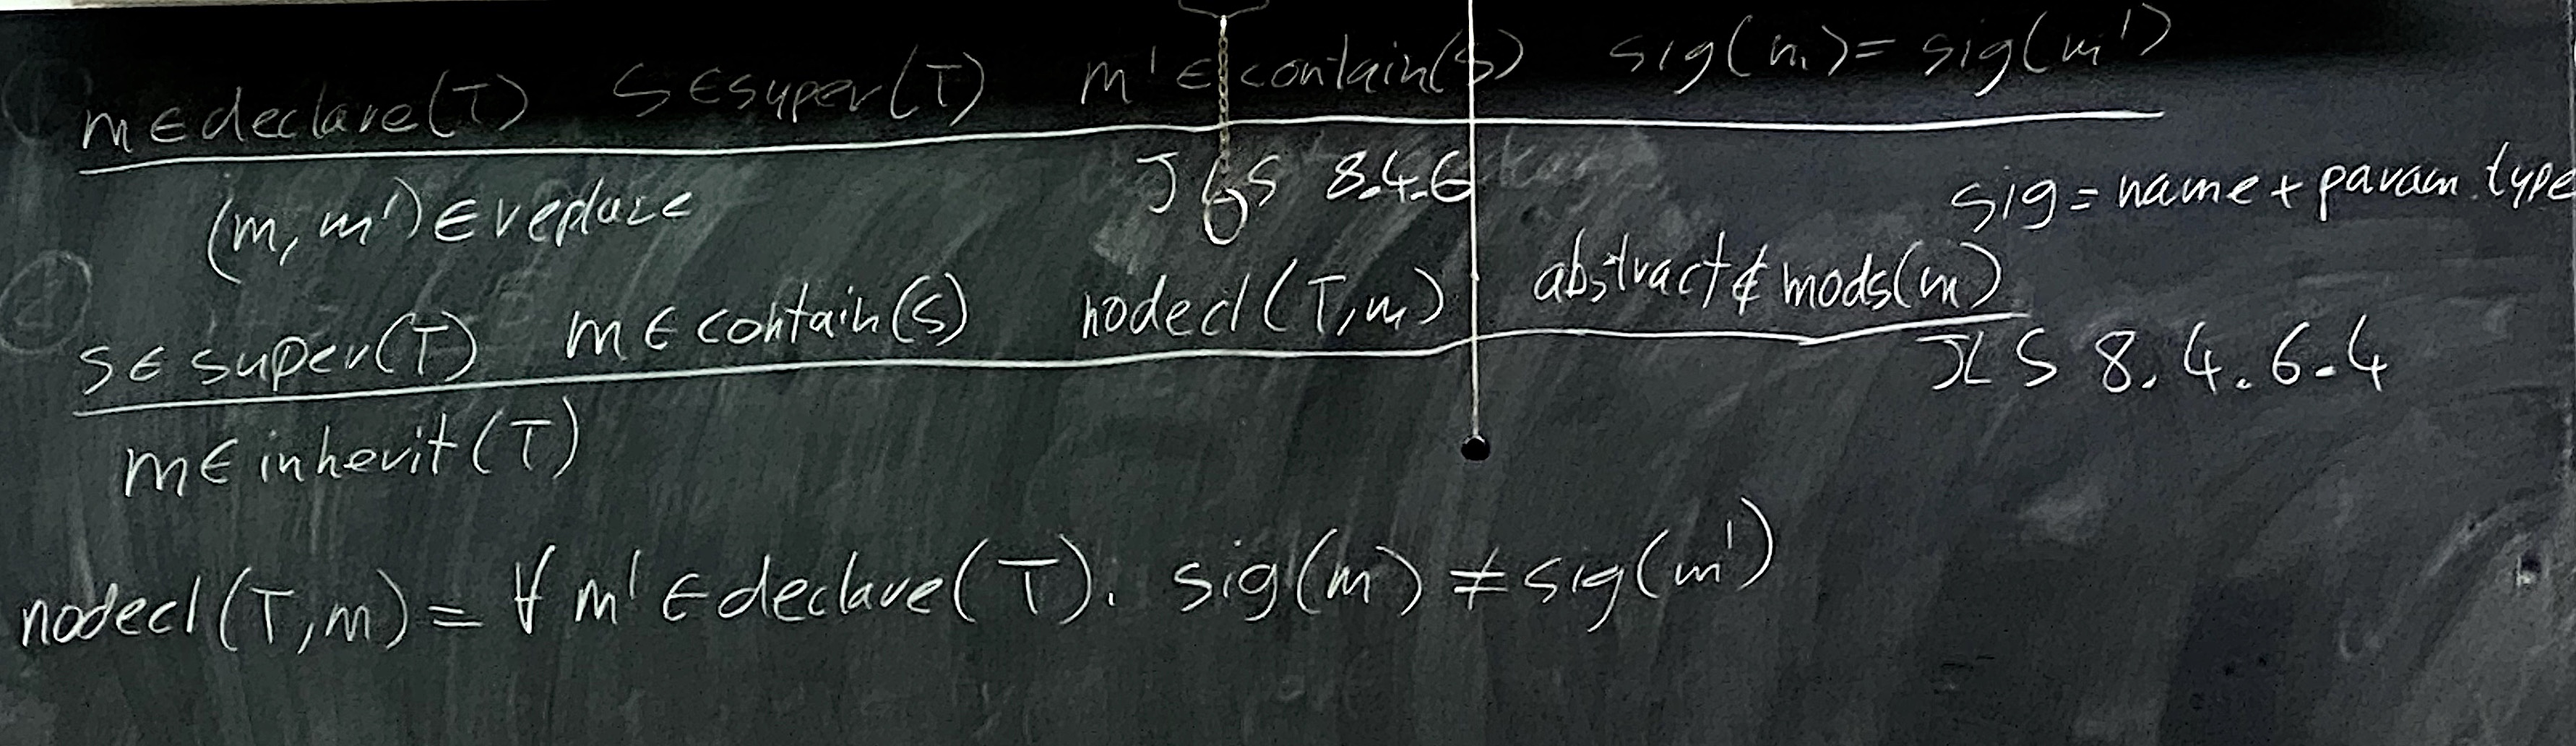
\includegraphics[scale=0.1]{11}
\end{center}
\end{itemize}a
\end{itemize}



\end{document}







